
\section{Issues and motivations (bis)}

Causal broadcast is a communication primitive that allows a process to send
messages to all processes of its distributed system (\REF). Message deliveries
follow the happen before relationship (\REF). If the sending of a message $m$
precedes the sending of a message $m'$ then all processes that deliver these two
messages need to deliver $m$ before $m'$. Otherwise they deliver them in any
order. Each process may receive a message multiple times but it delivers it
exactly once.

\PCBROADCAST (\REF) is a causal broadcast that improves state-of-the-art
approaches (\REF) by removing the need for piggybacking control information the
size of which is linear. It uses FIFO communications links for causal broadcast
and control messages to handle dynamicity.  Figure~\ref{fig:spaceproblem}
depicts its functioning while highlighting the problem. 



\begin{figure*}
  \begin{center}
    \subfloat[Part A][\label{fig:spaceproblemA}Process~B broadcasts $b$ along
    with control information $\langle B,\,1 \rangle$.]
    {
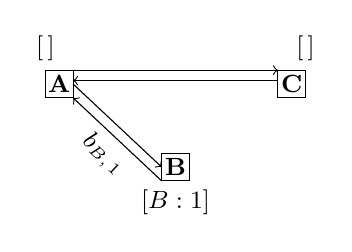
\begin{tikzpicture}[scale=1]
  
  \small
  
  \newcommand\X{210/5pt};
  \newcommand\Y{30pt};

  
  \draw[fill=white] (0*\X, 0*\Y) node{\textbf{A}} +(-5pt, -5pt) rectangle +(5pt, 5pt);
  \draw (-5+0*\X, 5+0*\Y) node[above]{$[\,]$};
  \draw[fill=white] (1*\X, -1*\Y) node{\textbf{B}} +(-5pt, -5pt) rectangle +(5pt, 5pt);
  \draw (1*\X, -5-1*\Y) node[below]{$[\bm{B:1}]$};
  \draw[fill=white] (2*\X,  0*\Y) node{\textbf{C}} +(-5pt, -5pt) rectangle +(5pt, 5pt);
  \draw (5+2*\X, 5+0*\Y) node[above]{$[\,]$};
  
  \draw[->](5+0*\X, 0*\Y) -- (-5+1*\X, -1*\Y); %% A->B
  \draw[<-](5+0*\X, -5+0*\Y) --
  node[sloped,below]{$\bm{b_{B,\,1}}$}
  (-5+1*\X, -5-1*\Y); %% A<-B
  
  \draw[->](5+0*\X, 5+0*\Y) -- (-5+2*\X, 5+0*\Y); % A->C
  \draw[<-](5+0*\X,  1.25+ 0*\Y) -- (-5+2*\X,  1.25+ 0*\Y); % A<-C
  
  % \draw[->,dashed](5+1*\X, -1*\Y) -- (-5+2*\X, 0*\Y); %% B<-C
  % \draw[->, dashed](5+1*\X, -5-1*\Y) -- (-5+2*\X, -5+0*\Y); %% B->C



\end{tikzpicture}}
    \hspace{10pt}
    \subfloat[Part B][\label{fig:spaceproblemB}Process~A receives, saves in its
    local vector, delivers and forwards
    $b$. Process~B wants to add Process~C in its direct neighbors for
    causal broadcast. It sends a control message $\pi$ to Process~C using 
    Process~A as mediator.]
    {
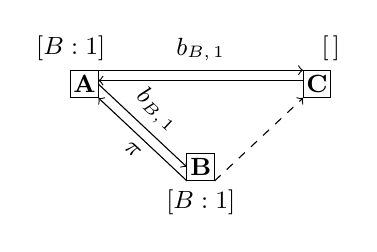
\begin{tikzpicture}[scale=1]
  
  \small
  
  \newcommand\X{210/5pt};
  \newcommand\Y{30pt};

  
  \draw[fill=white] (0*\X, 0*\Y) node{\textbf{A}} +(-5pt, -5pt) rectangle +(5pt, 5pt);
  \draw (-5+0*\X, 5+0*\Y) node[above]{$[\bm{B:1}]$};
  \draw[fill=white] (1*\X, -1*\Y) node{\textbf{B}} +(-5pt, -5pt) rectangle +(5pt, 5pt);
  \draw (1*\X, -5-1*\Y) node[below]{$[B:1]$};
  \draw[fill=white] (2*\X,  0*\Y) node{\textbf{C}} +(-5pt, -5pt) rectangle +(5pt, 5pt);
  \draw (5+2*\X, 5+0*\Y) node[above]{$[\,]$};
  
  \draw[->](5+0*\X, 0*\Y) -- 
  node[sloped,above]{$b_{B,\,1}$}
  (-5+1*\X, -1*\Y); %% A->B

  \draw[<-](5+0*\X, -5+0*\Y) --
  node[sloped, below]{$\bm{\pi}$}
  (-5+1*\X, -5-1*\Y); %% A<-B
  
  \draw[->](5+0*\X, 5+0*\Y) --
  node[sloped,above]{$b_{B,\,1}$}
  (-5+2*\X, 5+0*\Y); % A->C
  
  \draw[<-](5+0*\X,  1.25+ 0*\Y) -- (-5+2*\X,  1.25+ 0*\Y); % A<-C
  
  % \draw[->,dashed](5+1*\X, -1*\Y) -- (-5+2*\X, 0*\Y); %% B<-C
  \draw[->, dashed](5+1*\X, -5-1*\Y) -- (-5+2*\X, -5+0*\Y); %% B->C



\end{tikzpicture}}    
    \hspace{10pt}
    \subfloat[Part C][\label{fig:spaceproblemC}Process~A broadcasts $a$ along with
    control information $\langle A,\, 1 \rangle$. Then, it routes $\pi$ towards
    Process~C. Process~B receives $b$ but discards it, for it is already
    registered in Process~B's local vector.]
    {
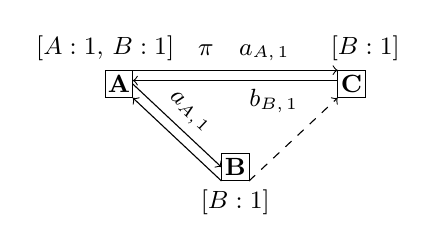
\begin{tikzpicture}[scale=1]
  
  \small
  
  \newcommand\X{210/5pt};
  \newcommand\Y{30pt};

  
  \draw[fill=white] (0*\X, 0*\Y) node{\textbf{A}} +(-5pt, -5pt) rectangle +(5pt, 5pt);
  \draw (-5+0*\X, 5+0*\Y) node[above]{$[\bm{A:1},\,B:1]$};
  \draw[fill=white] (1*\X, -1*\Y) node{\textbf{B}} +(-5pt, -5pt) rectangle +(5pt, 5pt);
  \draw (1*\X, -5-1*\Y) node[below]{$[B:1]$};
  \draw[fill=white] (2*\X,  0*\Y) node{\textbf{C}} +(-5pt, -5pt) rectangle +(5pt, 5pt);
  \draw (5+2*\X, 5+0*\Y) node[above]{$[\bm{B:1}]$};
  
  \draw[->](5+0*\X, 0*\Y) -- 
  node[sloped,above]{$\bm{a_{A,\,1}}$}
  (-5+1*\X, -1*\Y); %% A->B

  \draw[<-](5+0*\X, -5+0*\Y) --
  (-5+1*\X, -5-1*\Y); %% A<-B
  
  \draw[->](5+0*\X, 5+0*\Y) --
  node[above]{~~$\pi$~~~$\bm{a_{A,\,1}}$}
  (-5+2*\X, 5+0*\Y); % A->C
  
  \draw[<-](5+0*\X,  1.25+ 0*\Y) --
  node[below]{ ~ ~ ~ ~ ~$b_{B,\,1}$}
 (-5+2*\X,  1.25+ 0*\Y); % A<-C
  
  % \draw[->,dashed](5+1*\X, -1*\Y) -- (-5+2*\X, 0*\Y); %% B<-C
  \draw[->, dashed](5+1*\X, -5-1*\Y) -- (-5+2*\X, -5+0*\Y); %% B->C



\end{tikzpicture}}
    \hspace{10pt}
    \subfloat[Part D][\label{fig:spaceproblemD}Process~B and Process~C receive,
    save in their local vector, deliver and forward $a$. In addition, Process~B
    buffers $a$ to send it later to Process~C.]
    {
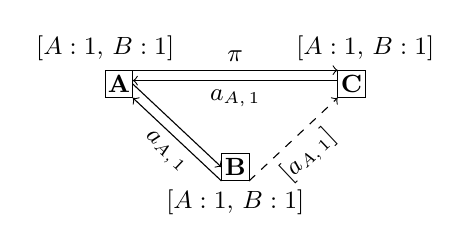
\begin{tikzpicture}[scale=1]
  
  \small
  
  \newcommand\X{210/5pt};
  \newcommand\Y{30pt};

  
  \draw[fill=white] (0*\X, 0*\Y) node{\textbf{A}} +(-5pt, -5pt) rectangle +(5pt, 5pt);
  \draw (-5+0*\X, 5+0*\Y) node[above]{$[A:1,\,B:1]$};
  \draw[fill=white] (1*\X, -1*\Y) node{\textbf{B}} +(-5pt, -5pt) rectangle +(5pt, 5pt);
  \draw (1*\X, -5-1*\Y) node[below]{$[\bm{A:1},\,B:1]$};
  \draw[fill=white] (2*\X,  0*\Y) node{\textbf{C}} +(-5pt, -5pt) rectangle +(5pt, 5pt);
  \draw (5+2*\X, 5+0*\Y) node[above]{$[\bm{A:1},\,B:1]$};
  
  \draw[->](5+0*\X, 0*\Y) -- 
  (-5+1*\X, -1*\Y); %% A->B

  \draw[<-](5+0*\X, -5+0*\Y) --
  node[sloped,below]{$\bm{a_{A,\,1}}$}
  (-5+1*\X, -5-1*\Y); %% A<-B
  
  \draw[->](5+0*\X, 5+0*\Y) --
  node[above]{$\pi$}
  (-5+2*\X, 5+0*\Y); % A->C
  
  \draw[<-](5+0*\X,  1.25+ 0*\Y) --
  node[below]{$\bm{a_{A,\,1}}$}
  (-5+2*\X,  1.25+ 0*\Y); % A<-C
  
  % \draw[->,dashed](5+1*\X, -1*\Y) -- (-5+2*\X, 0*\Y); %% B<-C
  \draw[->, dashed](5+1*\X, -5-1*\Y) --
  node[sloped, below]{$[a_{A,\,1}]$} (-5+2*\X, -5+0*\Y); %% B->C



\end{tikzpicture}}
    \hspace{10pt}
    \subfloat[Part E][\label{fig:spaceproblemE}Process~C receives $\pi$ and 
    replies $\rho$ to Process~B.]
    {
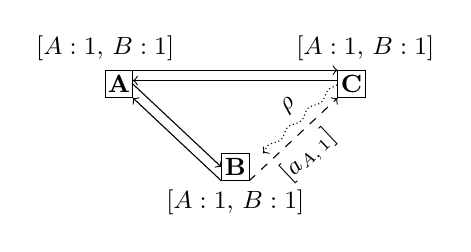
\begin{tikzpicture}[scale=1]
  
  \small
  
  \newcommand\X{210/5pt};
  \newcommand\Y{30pt};

  
  \draw[fill=white] (0*\X, 0*\Y) node{\textbf{A}} +(-5pt, -5pt) rectangle +(5pt, 5pt);
  \draw (-5+0*\X, 5+0*\Y) node[above]{$[A:1,\,B:1]$};
  \draw[fill=white] (1*\X, -1*\Y) node{\textbf{B}} +(-5pt, -5pt) rectangle +(5pt, 5pt);
  \draw (1*\X, -5-1*\Y) node[below]{$[A:1,\,B:1]$};
  \draw[fill=white] (2*\X,  0*\Y) node{\textbf{C}} +(-5pt, -5pt) rectangle +(5pt, 5pt);
  \draw (5+2*\X, 5+0*\Y) node[above]{$[A:1,\,B:1]$};
  
  \draw[->](5+0*\X, 0*\Y) -- 
  (-5+1*\X, -1*\Y); %% A->B

  \draw[<-](5+0*\X, -5+0*\Y) --
  (-5+1*\X, -5-1*\Y); %% A<-B
  
  \draw[->](5+0*\X, 5+0*\Y) --
  (-5+2*\X, 5+0*\Y); % A->C
  
  \draw[<-](5+0*\X,  1.25+ 0*\Y) --
  (-5+2*\X,  1.25+ 0*\Y); % A<-C
  
  % \draw[->,dashed](5+1*\X, -1*\Y) -- (-5+2*\X, 0*\Y); %% B<-C
 \draw[<-,densely dotted,decorate, decoration={snake, amplitude=0.3mm}](5+5+1*\X, 5+-1*\Y) -- 
 node[above, sloped]{$\bm{\rho}$}
 (-5+2*\X, 0*\Y);

  \draw[->, dashed](5+1*\X, -5-1*\Y) --
  node[sloped, below]{$[a_{A,\,1}]$} (-5+2*\X, -5+0*\Y); %% B->C



\end{tikzpicture}}
    \hspace{10pt}
    \subfloat[Part F][\label{fig:spaceproblemF}Process~B empties its buffer to
    Process~C. The latter will discard the message $a$, for it is already registered
    in Process~C's local vector]
    {
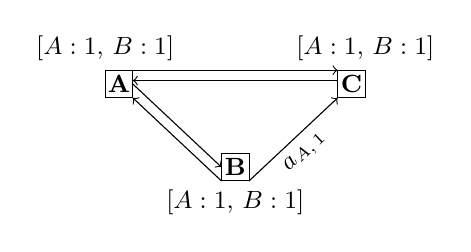
\begin{tikzpicture}[scale=1]
  
  \small
  
  \newcommand\X{210/5pt};
  \newcommand\Y{30pt};

  
  \draw[fill=white] (0*\X, 0*\Y) node{\textbf{A}} +(-5pt, -5pt) rectangle +(5pt, 5pt);
  \draw (-5+0*\X, 5+0*\Y) node[above]{$[A:1,\,B:1]$};
  \draw[fill=white] (1*\X, -1*\Y) node{\textbf{B}} +(-5pt, -5pt) rectangle +(5pt, 5pt);
  \draw (1*\X, -5-1*\Y) node[below]{$[A:1,\,B:1]$};
  \draw[fill=white] (2*\X,  0*\Y) node{\textbf{C}} +(-5pt, -5pt) rectangle +(5pt, 5pt);
  \draw (5+2*\X, 5+0*\Y) node[above]{$[A:1,\,B:1]$};
  
  \draw[->](5+0*\X, 0*\Y) -- 
  (-5+1*\X, -1*\Y); %% A->B

  \draw[<-](5+0*\X, -5+0*\Y) --
  (-5+1*\X, -5-1*\Y); %% A<-B
  
  \draw[->](5+0*\X, 5+0*\Y) --
  (-5+2*\X, 5+0*\Y); % A->C
  
  \draw[<-](5+0*\X,  1.25+ 0*\Y) --
  (-5+2*\X,  1.25+ 0*\Y); % A<-C
  
  % \draw[->,dashed](5+1*\X, -1*\Y) -- (-5+2*\X, 0*\Y); %% B<-C
  \draw[->](5+1*\X, -5-1*\Y) --
  node[sloped, below]{$\bm{a_{A,\,1}}$} (-5+2*\X, -5+0*\Y); %% B->C



\end{tikzpicture}}
    \caption{\label{fig:spaceproblem}\PCBROADCAST relies on vectors to deliver
      once and discard multiple receipts. The size of vectors increases linearly
      with the number of processes that ever broadcast a message.}
  \end{center}
\end{figure*}

\begin{figure*}
  \begin{center}
    \subfloat[Part A][\label{fig:counterproblemA}Process~B broadcasts the 
    message $b$ and expects to receive 1 copy of $b$.]
    {
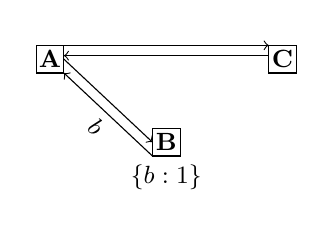
\begin{tikzpicture}[scale=1]
  
  \small
  
  \newcommand\X{210/5pt};
  \newcommand\Y{30pt};

  
  \draw[fill=white] (0*\X, 0*\Y) node{\textbf{A}} +(-5pt, -5pt) rectangle +(5pt, 5pt);
  \draw (-5+0*\X, 5+0*\Y) node[above]{$\varnothing$};
  \draw[fill=white] (1*\X, -1*\Y) node{\textbf{B}} +(-5pt, -5pt) rectangle +(5pt, 5pt);
  \draw (1*\X, -5-1*\Y) node[below]{$\{\bm{b:1}\}$};
  \draw[fill=white] (2*\X,  0*\Y) node{\textbf{C}} +(-5pt, -5pt) rectangle +(5pt, 5pt);
  \draw (5+2*\X, 5+0*\Y) node[above]{$\varnothing$};
  
  \draw[->](5+0*\X, 0*\Y) -- (-5+1*\X, -1*\Y); %% A->B
  \draw[<-](5+0*\X, -5+0*\Y) --
  node[sloped,below]{$\bm{b}$}
  (-5+1*\X, -5-1*\Y); %% A<-B
  
  \draw[->](5+0*\X, 5+0*\Y) -- (-5+2*\X, 5+0*\Y); % A->C
  \draw[<-](5+0*\X,  1.25+ 0*\Y) -- (-5+2*\X,  1.25+ 0*\Y); % A<-C
  
  % \draw[->,dashed](5+1*\X, -1*\Y) -- (-5+2*\X, 0*\Y); %% B<-C
  % \draw[->, dashed](5+1*\X, -5-1*\Y) -- (-5+2*\X, -5+0*\Y); %% B->C



\end{tikzpicture}}
    \hspace{10pt}
    \subfloat[Part B][\label{fig:counterproblemB}Process~A receives, delivers
    and forwards $b$. It expects 1 additional copy of $b$. Process~B wants to 
    add Process~C in its direct neighbors for causal broadcast. It sends a 
    control message $\pi$ to Process~C using Process~A as mediator.]
    {
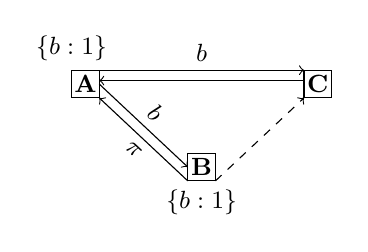
\begin{tikzpicture}[scale=1]
  
  \small
  
  \newcommand\X{210/5pt};
  \newcommand\Y{30pt};

  
  \draw[fill=white] (0*\X, 0*\Y) node{\textbf{A}} +(-5pt, -5pt) rectangle +(5pt, 5pt);
  \draw (-5+0*\X, 5+0*\Y) node[above]{$\{\bm{b:1}\}$};
  \draw[fill=white] (1*\X, -1*\Y) node{\textbf{B}} +(-5pt, -5pt) rectangle +(5pt, 5pt);
  \draw (1*\X, -5-1*\Y) node[below]{$\{b:1\}$};
  \draw[fill=white] (2*\X,  0*\Y) node{\textbf{C}} +(-5pt, -5pt) rectangle +(5pt, 5pt);
  \draw (5+2*\X, 5+0*\Y) node[above]{$\varnothing$};
  
  \draw[->](5+0*\X, 0*\Y) -- 
  node[sloped,above]{$b$}
  (-5+1*\X, -1*\Y); %% A->B

  \draw[<-](5+0*\X, -5+0*\Y) --
  node[sloped, below]{$\bm{\pi}$}
  (-5+1*\X, -5-1*\Y); %% A<-B
  
  \draw[->](5+0*\X, 5+0*\Y) --
  node[sloped,above]{$b$}
  (-5+2*\X, 5+0*\Y); % A->C
  
  \draw[<-](5+0*\X,  1.25+ 0*\Y) -- (-5+2*\X,  1.25+ 0*\Y); % A<-C
  
  % \draw[->,dashed](5+1*\X, -1*\Y) -- (-5+2*\X, 0*\Y); %% B<-C
  \draw[->, dashed](5+1*\X, -5-1*\Y) -- (-5+2*\X, -5+0*\Y); %% B->C



\end{tikzpicture}}
    \hspace{10pt}
    \subfloat[Part C][\label{fig:counterproblemC}Process~A broadcasts $a$. It 
    expects 2 copies. Process~B receives $b$ again, it does not expect any other 
    copy. Hence, it purges its local structure from $b$. Process~C receives, 
    delivers and forwards $b$. It does not expect additional copies.]
    {
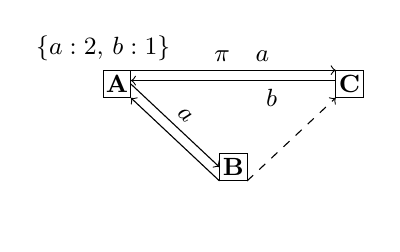
\begin{tikzpicture}[scale=1]
  
  \small
  
  \newcommand\X{210/5pt};
  \newcommand\Y{30pt};

  
  \draw[fill=white] (0*\X, 0*\Y) node{\textbf{A}} +(-5pt, -5pt) rectangle +(5pt, 5pt);
  \draw (-5+0*\X, 5+0*\Y) node[above]{$\{\bm{a:2},\,b:1\}$};
  \draw[fill=white] (1*\X, -1*\Y) node{\textbf{B}} +(-5pt, -5pt) rectangle +(5pt, 5pt);
  \draw (1*\X, -5-1*\Y) node[below]{$\bm{\varnothing}$\vphantom{$\{$}};
  \draw[fill=white] (2*\X,  0*\Y) node{\textbf{C}} +(-5pt, -5pt) rectangle +(5pt, 5pt);
  \draw (5+2*\X, 5+0*\Y) node[above]{$\varnothing$};
  
  \draw[->](5+0*\X, 0*\Y) -- 
  node[sloped,above]{$\bm{a}$}
  (-5+1*\X, -1*\Y); %% A->B

  \draw[<-](5+0*\X, -5+0*\Y) --
  (-5+1*\X, -5-1*\Y); %% A<-B
  
  \draw[->](5+0*\X, 5+0*\Y) --
  node[above]{~~$\pi$~~~$\bm{a}$}
  (-5+2*\X, 5+0*\Y); % A->C
  
  \draw[<-](5+0*\X,  1.25+ 0*\Y) --
  node[below]{ ~ ~ ~ ~ ~$b$}
 (-5+2*\X,  1.25+ 0*\Y); % A<-C
  
  % \draw[->,dashed](5+1*\X, -1*\Y) -- (-5+2*\X, 0*\Y); %% B<-C
  \draw[->, dashed](5+1*\X, -5-1*\Y) -- (-5+2*\X, -5+0*\Y); %% B->C



\end{tikzpicture}}
    \hspace{10pt}
    \subfloat[Part D][\label{fig:counterproblemD}Process~A receives, discards,
    and purges $b$. Process~B and Process~C receive, deliver, and forward $a$ but
    do not expect any additional copy. Process~B buffers $a$ to ensure the safety 
    of the new link.]
    {
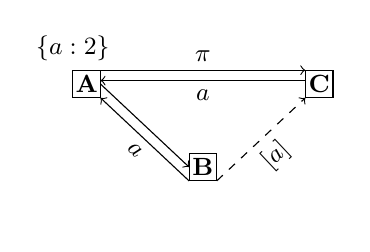
\begin{tikzpicture}[scale=1]
  
  \small
  
  \newcommand\X{210/5pt};
  \newcommand\Y{30pt};

  
  \draw[fill=white] (0*\X, 0*\Y) node{\textbf{A}} +(-5pt, -5pt) rectangle +(5pt, 5pt);
  \draw (-5+0*\X, 5+0*\Y) node[above]{$\{a:2\}$};
  \draw[fill=white] (1*\X, -1*\Y) node{\textbf{B}} +(-5pt, -5pt) rectangle +(5pt, 5pt);
  \draw (1*\X, -5-1*\Y) node[below]{$\varnothing$\vphantom{$\{$}};
  \draw[fill=white] (2*\X,  0*\Y) node{\textbf{C}} +(-5pt, -5pt) rectangle +(5pt, 5pt);
  \draw (5+2*\X, 5+0*\Y) node[above]{$\varnothing$};
  
  \draw[->](5+0*\X, 0*\Y) -- 
  (-5+1*\X, -1*\Y); %% A->B

  \draw[<-](5+0*\X, -5+0*\Y) --
  node[sloped,below]{$a$}
  (-5+1*\X, -5-1*\Y); %% A<-B
  
  \draw[->](5+0*\X, 5+0*\Y) --
  node[above]{$\pi$}
  (-5+2*\X, 5+0*\Y); % A->C
  
  \draw[<-](5+0*\X,  1.25+ 0*\Y) --
  node[below]{$a$}
  (-5+2*\X,  1.25+ 0*\Y); % A<-C
  
  % \draw[->,dashed](5+1*\X, -1*\Y) -- (-5+2*\X, 0*\Y); %% B<-C
  \draw[->, dashed](5+1*\X, -5-1*\Y) --
  node[sloped, below]{$[a]$} (-5+2*\X, -5+0*\Y); %% B->C



\end{tikzpicture}}
    \hspace{10pt}
    \subfloat[Part E][\label{fig:counterproblemE}Process~A receives and discards 
    two copies of $a$. It purges its local structure of $a$. Process~C receives
    $\pi$ and replies $\rho$ to Process~B.]
    {
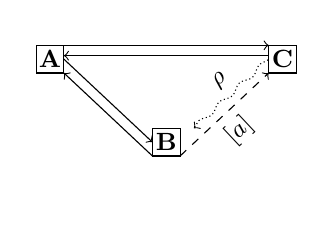
\begin{tikzpicture}[scale=1]
  
  \small
  
  \newcommand\X{210/5pt};
  \newcommand\Y{30pt};

  
  \draw[fill=white] (0*\X, 0*\Y) node{\textbf{A}} +(-5pt, -5pt) rectangle +(5pt, 5pt);
  \draw (-5+0*\X, 5+0*\Y) node[above]{$\varnothing$};
  \draw[fill=white] (1*\X, -1*\Y) node{\textbf{B}} +(-5pt, -5pt) rectangle +(5pt, 5pt);
  \draw (1*\X, -5-1*\Y) node[below]{$\varnothing$\vphantom{$\{$}};
  \draw[fill=white] (2*\X,  0*\Y) node{\textbf{C}} +(-5pt, -5pt) rectangle +(5pt, 5pt);
  \draw (5+2*\X, 5+0*\Y) node[above]{$\varnothing$};
  
  \draw[->](5+0*\X, 0*\Y) -- 
  (-5+1*\X, -1*\Y); %% A->B

  \draw[<-](5+0*\X, -5+0*\Y) --
  (-5+1*\X, -5-1*\Y); %% A<-B
  
  \draw[->](5+0*\X, 5+0*\Y) --
  (-5+2*\X, 5+0*\Y); % A->C
  
  \draw[<-](5+0*\X,  1.25+ 0*\Y) --
  (-5+2*\X,  1.25+ 0*\Y); % A<-C
  
  % \draw[->,dashed](5+1*\X, -1*\Y) -- (-5+2*\X, 0*\Y); %% B<-C
 \draw[<-,densely dotted,decorate, decoration={snake, amplitude=0.3mm}](5+5+1*\X, 5+-1*\Y) -- 
 node[above, sloped]{$\bm{\rho}$}
 (-5+2*\X, 0*\Y);

  \draw[->, dashed](5+1*\X, -5-1*\Y) --
  node[sloped, below]{$[a]$} (-5+2*\X, -5+0*\Y); %% B->C



\end{tikzpicture}}
    \hspace{10pt}
    \subfloat[Part F][\label{fig:counterproblemF}Process~B empties its buffer
    to Process~C. Not only Process~C mistakes $a$ for a new message and delivers it 
    again, but it has cascading effects due to the forwarding.]
    {
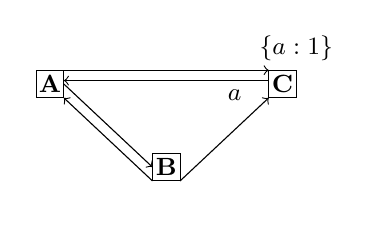
\begin{tikzpicture}[scale=1]
  
  \small
  
  \newcommand\X{210/5pt};
  \newcommand\Y{30pt};

  
  \draw[fill=white] (0*\X, 0*\Y) node{\textbf{A}} +(-5pt, -5pt) rectangle +(5pt, 5pt);
  \draw (-5+0*\X, 5+0*\Y) node[above]{$\varnothing$};
  \draw[fill=white] (1*\X, -1*\Y) node{\textbf{B}} +(-5pt, -5pt) rectangle +(5pt, 5pt);
  \draw (1*\X, -5-1*\Y) node[below]{$\varnothing$\vphantom{$\{$}};
  \draw[fill=white] (2*\X,  0*\Y) node{\textbf{C}} +(-5pt, -5pt) rectangle +(5pt, 5pt);
  \draw (5+2*\X, 5+0*\Y) node[above]{$\{\bm{a:1}\}$};
  
  \draw[->](5+0*\X, 0*\Y) -- 
  (-5+1*\X, -1*\Y); %% A->B

  \draw[<-](5+0*\X, -5+0*\Y) --
  (-5+1*\X, -5-1*\Y); %% A<-B
  
  \draw[->](5+0*\X, 5+0*\Y) --
  (-5+2*\X, 5+0*\Y); % A->C
  
  \draw[<-](5+0*\X,  1.25+ 0*\Y) --
  node[sloped, below]{ ~ ~ ~ ~ ~ ~ ~ ~~$\bm{a}$}
  (-5+2*\X,  1.25+ 0*\Y); % A<-C
  
  % \draw[->,dashed](5+1*\X, -1*\Y) -- (-5+2*\X, 0*\Y); %% B<-C
  \draw[->](5+1*\X, -5-1*\Y) --
  (-5+2*\X, -5+0*\Y); %% B->C



\end{tikzpicture}}
    \caption{\label{fig:counterproblem}Using counters to discard multiple receipts
      is more efficient in terms of memory usage but fails in dynamic systems.}
  \end{center}
\end{figure*}

%%% Local Variables:
%%% mode: latex
%%% TeX-master: "../paper"
%%% End:
